\section{第一类算子方程}
\label{sec:opeq-first-kind}

测量仪器往往不直接给出我们想知道的函数，而是给出它经过平均、平滑或累积后的结果。若这个过程是线性的，就可以写成一个算子$K$作用在未知函数$f$上，测得的输出是$g$。从$g$推回$f$，就是求解一个算子方程。本节固定Hilbert空间之间的紧算子，先说明“有解”和“唯一”分别对应算子的哪个对象，再借助奇异系统把这两个条件写成可以逐项核对的系数条件。

\paragraph{方程与两个基本问题}
设$H_1,H_2$是同一数域$\mathbb F$（$\mathbb R$或$\mathbb C$）上的Hilbert空间，$K\in\mathcal B(H_1,H_2)$，$g\in H_2$已知。复内积沿用对第一个变量共轭线性、对第二个变量线性的约定。

\begin{definition}[第一类算子方程]
\label{def:opeq-first-kind}
给定$K\in\mathcal B(H_1,H_2)$与$g\in H_2$，求$f\in H_1$使
\begin{equation}
  Kf=g ,
  \label{eq:opeq-first-kind}
\end{equation}
称为\term{第一类算子方程}（operator equation of the first kind）。$K$为积分算子时，也称为第一类积分方程。
\end{definition}

这里未知函数只出现在算子里面，方程等于问：$g$是不是$K$的一个输出。由此立即得到两条判别。方程~\eqref{eq:opeq-first-kind}有解当且仅当$g\in\operatorname{Ran}K$。若$f_0$是一个解，则$f$是解当且仅当$K(f-f_0)=0$，所以全部解组成$f_0+\ker K$；解唯一当且仅当$\ker K=\{0\}$。存在性问的是输出空间里的一个集合，唯一性问的是输入空间里的一个子空间，两者需要分别核对。

\paragraph{秩二积分算子的例子}
取$H=L^2([-1,1],\mu)$，其中$\mathrm d\mu=\mathrm dz/2$，在其上定义核为$1+xz$的积分算子
\begin{equation}
  (Tf)(x)=\int_{-1}^{1}(1+xz)f(z)\,\frac{\mathrm dz}2
  =\langle 1,f\rangle+x\,\langle z,f\rangle ,
  \label{eq:opeq-rank-two}
\end{equation}
这里核是实值的，$\langle 1,f\rangle$与$\langle z,f\rangle$分别是$f$与常函数$1$、一次函数$z$的内积。在这个测度下$\lVert1\rVert^2=1$，$\lVert x\rVert^2=\int_{-1}^1x^2\,\mathrm dx/2=1/3$，而$\langle1,x\rangle=0$。于是任意$f$可以唯一地写成$f=\alpha+\beta x+h$，其中$h$与$1,x$都正交，代入得
\[
  Tf=\alpha+\frac{\beta}{3}x .
\]
$T$的像是二维子空间$\operatorname{span}\{1,x\}$，零空间是$\{1,x\}$的正交补，后者是无限维的；例如$x^2-1/3$就在其中，因为它与$1$和$x$都正交。

因此第一类方程$Tf=g$只在$g=a+bx$时有解。比较系数得$\alpha=a$、$\beta=3b$，而$h$完全不受约束：
\[
  f=a+3bx+h,\qquad h\perp1,\ h\perp x .
\]
解一旦存在就有无穷多个，差别正是零空间中的任意元素。若$g$含有$x^2$这样的成分，无论怎样选$f$都得不到$g$：$T$把与$1,x$正交的方向全部压成零，这些方向上的信息在输出中已经丢失。

\paragraph{奇异系统下的系数关系}
对一般的紧算子，像和零空间不再这样一目了然。第~\ref{chap:operator-spectra}章为两个Hilbert空间之间的紧算子$K$构造了奇异系统：正数$\sigma_1\geq\sigma_2\geq\cdots>0$（有限个或可数无穷个，后者有$\sigma_j\to0$），$H_1$中的标准正交系$(v_j)$与$H_2$中的标准正交系$(u_j)$，使
\begin{equation}
  Kx=\sum_j\sigma_j\langle v_j,x\rangle u_j ,\qquad K^*u_j=\sigma_jv_j ,
  \label{eq:opeq-svd}
\end{equation}
并且$(v_j)$的闭线性张成是$(\ker K)^\perp$，$(u_j)$的闭线性张成是$\overline{\operatorname{Ran}K}$。第~\ref{chap:linear-operators}章又给出$\overline{\operatorname{Ran}K}=(\ker K^*)^\perp$。下面只用到这几条结论。

若$Kf=g$，对每个$j$取$u_j$与方程两边作内积，并把$K$移到另一侧：
\[
  \langle u_j,g\rangle=\langle u_j,Kf\rangle=\langle K^*u_j,f\rangle=\sigma_j\langle v_j,f\rangle .
\]
解在方向$v_j$上的系数因此被数据唯一确定为$\langle u_j,g\rangle/\sigma_j$。这一关系把方程拆成了可数个标量方程，但也提出了一个新要求：这些系数必须平方可和，拼起来的级数才代表$H_1$中的元素。

\begin{theorem}[第一类方程的可解条件与最小范数解]
\label{thm:opeq-picard}
设$K:H_1\to H_2$为紧算子，奇异系统如式~\eqref{eq:opeq-svd}。方程$Kf=g$有解，当且仅当以下两条同时成立：
\begin{equation}
  g\perp\ker K^* ,\qquad
  \sum_j\frac{\lvert\langle u_j,g\rangle\rvert^2}{\sigma_j^2}<\infty .
  \label{eq:opeq-picard}
\end{equation}
此时
\[
  f^\dagger=\sum_j\frac{\langle u_j,g\rangle}{\sigma_j}v_j
\]
是方程在$(\ker K)^\perp$中唯一的解，全部解为$f^\dagger+\ker K$，并且$f^\dagger$是范数最小的解。
\end{theorem}

\begin{proof}
必要性。若$Kf=g$，则$g\in\operatorname{Ran}K\subseteq(\ker K^*)^\perp$，第一条成立。由上面的系数关系和Bessel不等式，
\[
  \sum_j\frac{\lvert\langle u_j,g\rangle\rvert^2}{\sigma_j^2}=\sum_j\lvert\langle v_j,f\rangle\rvert^2\leq\lVert f\rVert^2<\infty ,
\]
第二条成立。

充分性。第二条说明$f^\dagger$的系数平方可和，所以级数在$H_1$中按范数收敛，且$f^\dagger$属于$(v_j)$的闭张成$(\ker K)^\perp$。$K$连续，可以逐项作用；由$Kv_j=\sigma_ju_j$得
\[
  Kf^\dagger=\sum_j\langle u_j,g\rangle u_j ,
\]
这是$g$在$(u_j)$的闭张成上的正交投影。这个闭张成等于$\overline{\operatorname{Ran}K}=(\ker K^*)^\perp$，第一条说明$g$就在其中，所以投影等于$g$本身，即$Kf^\dagger=g$。

解的结构。全部解为$f^\dagger+\ker K$。若$f_1,f_2$都是$(\ker K)^\perp$中的解，则$f_1-f_2$同时属于$\ker K$与$(\ker K)^\perp$，只能为零。对任意解$f=f^\dagger+h$，$h\in\ker K$与$f^\dagger$正交，由勾股定理$\lVert f\rVert^2=\lVert f^\dagger\rVert^2+\lVert h\rVert^2\geq\lVert f^\dagger\rVert^2$。
\end{proof}

式~\eqref{eq:opeq-picard}中的第二个条件称为\term{Picard条件}（Picard condition），$f^\dagger$称为方程的最小范数解。两个条件分工不同。第一个只说明$g$落在像的闭包里，也就是$g$能被输出任意逼近；第二个才保证形式上的逆系数真正拼成输入空间中的元素。$K$只有有限个正奇异值时，第二个条件自动成立，只剩第一个；在秩二的例子中，$T$自伴且奇异值为$1$与$1/3$，对$g=a+bx$得$f^\dagger=a+3bx$，正是全部解中零空间分量为零的那一个。

\paragraph{像的闭包不等于像}
奇异值无限多时，两个条件确实不同。最简单的例子是$\ell^2$上的对角算子$A(x_n)=(x_n/n)$。它自伴、单射，$\ker A^*=\{0\}$，第一个条件对所有数据成立；奇异值为$1/n$，Picard条件化为$\sum_nn^2\lvert g_n\rvert^2<\infty$。取$g^{(1)}_n=1/n^2$，形式解系数为$1/n$，平方可和，方程有解$(1/n)$。取$g^{(2)}_n=1/n$，它本身平方可和，形式解系数却恒为$1$，所以$g^{(2)}$不在像中。图~\ref{fig:opeq-picard-coefficients}比较了这两组数据。

\begin{figure}[!htb]
  \centering
  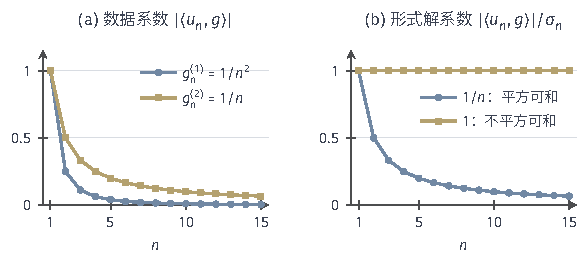
\includegraphics[width=99.6mm]{figures/02-abstract-mathematics/03-function-spaces/tikz/c3-picard-coefficients/figure.pdf}
  \caption{$\ell^2$上$A(x_n)=(x_n/n)$的Picard条件。(a)两组数据的系数$1/n^2$与$1/n$，都平方可和，都与$\ker A^*=\{0\}$正交。(b)除以奇异值$\sigma_n=1/n$后的形式解系数：前者为$1/n$，平方可和，方程可解；后者恒为$1$，不平方可和，方程无解。}
  \label{fig:opeq-picard-coefficients}
\end{figure}

函数空间中有同样的现象。在$L^2(0,1)$上考虑累积积分
\[
  (Vf)(x)=\int_0^xf(t)\,\mathrm dt .
\]
由Fubini定理交换积分次序，
\begin{equation*}
\langle g,Vf\rangle=\int_0^1\overline{g(x)}\int_0^xf(t)\,\mathrm dt\,\mathrm dx=\int_0^1\Bigl(\int_t^1\overline{g(x)}\,\mathrm dx\Bigr)f(t)\,\mathrm dt,
\end{equation*}
所以伴随为$(V^*g)(t)=\int_t^1g(x)\,\mathrm dx$。若$Vf=0$，则$f$在每个区间$[0,x]$上的积分为零，从而在每个子区间上的积分为零，$f=0$几乎处处；同理$V^*$也是单射。于是$\ker V=\ker V^*=\{0\}$，$V$的像在$L^2(0,1)$中稠密。

$V$的奇异系统可以直接写出。记$\omega_k=(k-\frac12)\pi$，$k=1,2,\ldots$，令
\[
  v_k(x)=\sqrt2\cos\omega_kx,\qquad u_k(x)=\sqrt2\sin\omega_kx,\qquad \sigma_k=\frac1{\omega_k}.
\]
直接积分得$Vv_k=\sqrt2\sin(\omega_kx)/\omega_k=\sigma_ku_k$；又由$\cos\omega_k=0$，$V^*u_k=\sqrt2\bigl(\cos\omega_kx-\cos\omega_k\bigr)/\omega_k=\sigma_kv_k$。由$\sin2\omega_k=0$可验证$(v_k)$与$(u_k)$各自标准正交。

还要说明这些就是全部奇异方向。$V^*V$是紧自伴算子且为单射，由第~\ref{chap:operator-spectra}章的谱分解，它的非零特征方向张成整个$L^2(0,1)$。若$V^*Vf=\mu f$，$\mu>0$，令$y=V^*Vf$，则$y(x)=\int_x^1\int_0^tf$，于是$y(1)=0$，$y'(x)=-\int_0^xf$，$y'(0)=0$。$f=y/\mu$连续，故$y$二阶连续可微且$y''=-f=-y/\mu$。满足$y'(0)=0$的解为$y=c\cos(x/\sqrt\mu)$，再由$y(1)=0$得$1/\sqrt\mu=\omega_k$。因此特征值为$\sigma_k^2$，每个特征空间由$v_k$张成，$(v_k)$是$L^2(0,1)$的标准正交基。

现在取数据$g=1$。由$\ker V^*=\{0\}$，它满足第一个条件。系数为
\[
  \langle u_k,1\rangle=\sqrt2\int_0^1\sin\omega_kx\,\mathrm dx=\frac{\sqrt2(1-\cos\omega_k)}{\omega_k}=\sqrt2\,\sigma_k ,
\]
形式解系数恒为$\sqrt2$，Picard条件不成立，所以$1\notin\operatorname{Ran}V$。这与直接观察一致：$Vf$总有在$0$处取零的连续代表，而常函数$1$的连续代表在$0$处取$1$，两个连续函数若几乎处处相等就处处相等。

$1$能被输出逼近，逼近的代价是输入越来越大。取$f_n=n\mathbf 1_{[0,1/n]}$，则$(Vf_n)(x)=\min\{nx,1\}$，
\[
  \lVert Vf_n-1\rVert^2=\int_0^{1/n}(1-nx)^2\,\mathrm dx=\frac1{3n}\to0,\qquad \lVert f_n\rVert^2=n\to\infty .
\]
输出误差趋于零时，产生这些输出的输入并不收敛，它们的范数无界。像的闭包里多出来的元素，正是只能这样“追到”而不能真正达到的数据。

\paragraph{Picard条件与求导}
对一般数据，$V$的Picard条件有一个熟悉的含义。设$g$有绝对连续的代表，$g(0)=0$且$g'\in L^2(0,1)$。分部积分，并利用$\cos\omega_k=0$与$g(0)=0$消去边界项：
\[
  \langle u_k,g\rangle=\Bigl[-\frac{\sqrt2\cos\omega_kx}{\omega_k}g(x)\Bigr]_0^1+\frac1{\omega_k}\int_0^1\sqrt2\cos(\omega_kx)\,g'(x)\,\mathrm dx=\sigma_k\langle v_k,g'\rangle .
\]
这里$g$取实值；复值时对实部、虚部分别计算即可。于是Picard级数等于$\sum_k\lvert\langle v_k,g'\rangle\rvert^2=\lVert g'\rVert^2<\infty$，最小范数解就是$f^\dagger=g'$。反过来，若$Vf=g$，则$g$绝对连续、$g(0)=0$且$g'=f$几乎处处。所以$\operatorname{Ran}V$恰好由这样的函数组成，求解第一类方程$Vf=g$就是对数据求导。

这个例子把前面的两个条件落到了具体的函数性质上：$g\perp\ker V^*$对所有$L^2$函数成立，几乎不提供信息；Picard条件则要求数据在$0$处的值合适并具有平方可积的导数。数据的这种正则性正是由奇异值趋于零的速度决定的，它将在第~\ref{sec:opeq-stability}节中重新出现，成为误差放大的来源。
